\documentclass[11pt]{article}

\usepackage[margin=1in]{geometry}
\usepackage[utf8]{inputenc}
\usepackage[T1]{fontenc}
\usepackage{amsmath,amssymb,amsthm}
\usepackage{booktabs}
\usepackage{graphicx}
\usepackage{natbib}
\usepackage{xcolor}
\usepackage[colorlinks=true, citecolor=blue, linkcolor=black, urlcolor=blue]{hyperref}
\usepackage{enumitem}
\setlist{nosep}
\emergencystretch=1.5em

\newcommand{\E}{\mathbb{E}}
\newcommand{\R}{\mathbb{R}}
\newcommand{\res}{\operatorname{res}}
\newcommand{\todo}[1]{\textcolor{red}{[#1]}}

\newtheorem{proposition}{Proposition}

\title{Perfect Foresight Is Almost Enough:\\ Risk Corrections in Function Space for Nonlinear New Keynesian Models\\[0.6em] {\large\bfseries Extended abstract}}
\author{Jan Rosa\thanks{OECD, \texttt{jan.rosa@oecd.org}. The opinions expressed and arguments employed in this paper are solely those of the authors and do not necessarily reflect the official views of the OECD or of its member states.}
\and Mahdi Ebrahimi Kahou\thanks{Bowdoin College.}
\and Jes\'us Fern\'andez-Villaverde\thanks{University of Pennsylvania.}}
\date{\today}

\begin{document}
\maketitle

\section{Introduction}
This paper proposes a new method for solving dynamic stochastic general 
equilibrium (DSGE) models: functional perturbation around the solution of 
a simplified deterministic model. Standard perturbation methods 
\citep{schmitt2004solving, fernandez2016solution} approximate 
policy functions by expanding them around a single point: 
the deterministic steady state. In contrast, we perturb around the 
full nonlinear solution of a simplified deterministic model, which can 
often be computed efficiently and accurately using deep 
learning or kernel methods, as demonstrated by 
\citet{kahou2024spooky, kahou2026kernel}. 

\paragraph{Contribution} Our contributions are threefold. First, under regularity
conditions on the equilibrium in a normed space, the deterministic solution
is close to the full stochastic solution, with a distance in norm of the
order of the variance of the largest shock in the model. Second,
starting from the deterministic solution, we propose a Newton--Kantorovich
algorithm that converges quickly to the stochastic solution. Third, to demonstrate
the method, we solve nonlinear New Keynesian models with capital accumulation under
both Rotemberg and Calvo pricing. The Calvo version with capital is notoriously nonlinear, and to the
best of our knowledge no global solution of it exists: existing solutions rely
on perturbation around the steady state, and global methods adopt Rotemberg
pricing or drop capital.



\paragraph{Intuition of the paper} The first step of our approach is to
learn the solution of the deterministic problem. This solution already contains
most of the information about the solution of the stochastic problem: the only
missing element is the effect of uncertainty. The second step learns this missing
element, which explains the fast convergence of our method.
The deterministic solution also provides something subtler.
Sampling the state space is challenging even in moderate
dimension \citep{kahou2021exploiting, fernandez2026taming}, and more so in highly nonlinear problems. Simulating the
deterministic solution under the calibrated shocks delivers a region of the state space that is close, although not identical, to
the region the stochastic economy visits.
This also contributes to the robustness and efficiency of our method.



\paragraph{Why start from the deterministic solution?} Three properties
of the deterministic solution, documented by \citet{kahou2024spooky, kahou2026kernel}
for neural networks and kernel machines, motivate this choice. First, the deterministic solution can be
computed accurately and cheaply, because the deterministic
problem is the simpler one. Second, through implicit or
explicit regularization of the solution paths, the solution automatically satisfies
the transversality and no-Ponzi conditions. This is crucial for
problems with hysteresis, which are common in growth
models \citep{skiba1978optimal, azariadis1990threshold}
and in open-economy models \citep{mendoza2010sudden, mendoza2020fipit}.
Third, because the transversality conditions are what make the equilibrium
path stable, a solution that satisfies them is stable and errors do not accumulate along
the dynamics. This error accumulation problem is more severe in highly
nonlinear models, such as the ones we study in this paper.\footnote{This is a well-known
problem in DSGE models, and fixes specific to each solution method
have been proposed, for instance pruning
in higher-order perturbation methods \citep{andreasen2018pruned}.}


\paragraph{Related works} Our approach is related 
to, but distinct from, the sequence-space methods 
of \citet{auclert2021sequence}. Whereas sequence-space 
methods use functional perturbations to approximate equilibrium objects,
 we use them to solve for the stochastic recursive equilibrium of 
 the entire economy across the state space.

\paragraph{Application} We apply the method to a New Keynesian model with 
capital under both Calvo and Rotemberg pricing. With a high elasticity of 
substitution, the Calvo pricing block is known to be strongly nonlinear 
\citep{ascari2014macroeconomics}: the reset-price and price-dispersion 
recursions have singularities a few percentage points above the inflation target.
We demonstrate that the Newton--Kantorovich iteration delivers stochastic 
policy functions whose equilibrium residuals are close to numerical zero 
along impulse responses and simulated paths, even in this case.



\section{Model and parametrization}

We use a standard New Keynesian economy with capital and Calvo pricing. To keep the exposition short, we do not add the standard shocks and mechanisms of medium-sized models (habits, investment adjustment costs, variable utilization, sticky wages, fiscal policy); the method does not depend on them.

\paragraph{Households.} A representative household maximizes
$\E_0 \sum_{t=0}^{\infty} \beta^t \big[ \log c_t - \psi\, l_t^{1+\eta}/(1+\eta) \big]$
subject to $c_t + k_t + b_{t+1}/p_t = w_t l_t + (1 + r_t - \delta) k_{t-1} + R_{t-1} b_t/p_t + T_t + F_t$. It saves in physical capital $k_t$ (rental rate $r_t$, depreciation $\delta$) and in nominal bonds $b_{t+1}$ (gross rate $R_t$). With $\lambda_t = 1/c_t$ the first-order conditions are
\begin{equation}
\psi l_t^{\eta} = \lambda_t w_t, \qquad
\lambda_t = \beta\, \E_t\!\left[ \lambda_{t+1} \frac{R_t}{\Pi_{t+1}} \right], \qquad
\lambda_t = \beta\, \E_t\!\left[ \lambda_{t+1} (1 + r_{t+1} - \delta) \right],
\label{eq:hh}
\end{equation}
where $\Pi_t = p_t/p_{t-1}$ is gross inflation.

\paragraph{Firms.} A competitive final-good producer aggregates intermediate varieties with elasticity of substitution $\epsilon$. Intermediate producer $i$ has the technology $y_{it} = e^{z_t} k_{it-1}^{\alpha} l_{it}^{1-\alpha}$ and rents inputs at $w_t$ and $r_t$, so that the real marginal cost is common across firms, $\mathrm{mc}_t = (1-\alpha)^{-(1-\alpha)} \alpha^{-\alpha}\, w_t^{1-\alpha} r_t^{\alpha} e^{-z_t}$. Prices are set \`a la Calvo: each period a fraction $1-\theta$ of firms resets its price. The optimal reset price relative to the price level, $\Pi_t^* = p_t^*/p_t$, is characterized by two auxiliary variables, the discounted sums of marginal costs and of revenues of the price setters,
\begin{equation}
g^1_t = \lambda_t\, \mathrm{mc}_t\, y_t + \beta\theta\, \E_t\!\left[ \Pi_{t+1}^{\epsilon} g^1_{t+1} \right], \qquad
g^2_t = \lambda_t\, \Pi^*_t\, y_t + \beta\theta\, \E_t\!\left[ \Pi_{t+1}^{\epsilon-1} \frac{\Pi^*_t}{\Pi^*_{t+1}}\, g^2_{t+1} \right], \qquad
\epsilon\, g^1_t = (\epsilon - 1)\, g^2_t,
\label{eq:calvo}
\end{equation}
and by the price index $1 = \theta \Pi_t^{\epsilon-1} + (1-\theta) (\Pi^*_t)^{1-\epsilon}$. Price dispersion $v_t = \int_0^1 (p_{it}/p_t)^{-\epsilon}\, di$ lowers aggregate supply, $y_t = e^{z_t} k_{t-1}^{\alpha} l_t^{1-\alpha} / v_t$, and evolves as $v_t = \theta \Pi_t^{\epsilon} v_{t-1} + (1-\theta) (\Pi^*_t)^{-\epsilon}$.

\paragraph{Monetary policy and shocks.} The central bank follows a Taylor rule that responds to inflation and to output \emph{growth},
\begin{equation}
R_t = R \left( \frac{\Pi_t}{\Pi} \right)^{\gamma_\Pi} \left( \frac{y_t}{y_{t-1}} \right)^{\gamma_{\Delta y}} e^{\xi_t},
\qquad
z_t = \rho z_{t-1} + \sigma_z \varepsilon_{z,t}, \qquad
\xi_t = \rho_m \xi_{t-1} + \sigma_m \varepsilon_{m,t},
\label{eq:taylor}
\end{equation}
with $\varepsilon_{z,t}, \varepsilon_{m,t} \sim \mathcal{N}(0,1)$. 

\paragraph{Market clearing.} $c_t + k_t = y_t + (1-\delta) k_{t-1}$.

\paragraph{Recursive formulation.} The state is $s_t = (z_t,\, k_{t-1},\, \xi_t,\, v_{t-1},\, y_{t-1})$ and the policy is $f(s_t) = (k_t,\, l_t,\, \Pi_t,\, g^1_t)$. Given $s_t$ and $f(s_t)$ every other date-$t$ object follows in closed form: $\Pi^*_t$ from the price index, $v_t$, $y_t$, $c_t$ from market clearing, $\lambda_t$, $w_t$, $r_t$, $\mathrm{mc}_t$, $R_t$, and $g^2_t$ from the reset-price condition. Market clearing therefore never appears as a residual. The four remaining conditions are the two Euler equations in \eqref{eq:hh} and the two Calvo recursions in \eqref{eq:calvo}; each is a ratio $N/D$ that equals one at the solution, and we take the residual as $\log(D/N)$.

Explicitly, for a candidate policy $f$ and a state $s = (z, k, \xi, v_{-1}, y_{-1})$, let $(k', l, \Pi, g^1) = f(s)$ and let $c, \lambda, y, v, \mathrm{mc}, r, R, \Pi^*, g^2$ be the date-$t$ objects recovered from them as above. The successor state under the innovation $\varepsilon = (\varepsilon_z, \varepsilon_m)$ is
\begin{equation}
s'(\varepsilon) = \big( \rho z + \sigma_z \varepsilon_z,\ k',\ \rho_m \xi + \sigma_m \varepsilon_m,\ v,\ y \big),
\label{eq:successor}
\end{equation}
and primed objects ($\lambda', \Pi', r', g^{1\prime}, g^{2\prime}, \Pi^{*\prime}$) are the same recovered quantities evaluated at $s'(\varepsilon)$ under the policy $f(s'(\varepsilon))$. The residual vector at $s$ is
\begin{equation}
l(\sigma, f)(s) =
\begin{pmatrix}
\log \lambda - \log\Big( \beta\, \E_\varepsilon\big[ R\, \lambda' / \Pi' \big] \Big)\\[0.4em]
\log \lambda - \log\Big( \beta\, \E_\varepsilon\big[ \lambda' (1 + r' - \delta) \big] \Big)\\[0.4em]
\log g^1 - \log\Big( \lambda\, \mathrm{mc}\, y + \beta\theta\, \E_\varepsilon\big[ \Pi'^{\epsilon} g^{1\prime} \big] \Big)\\[0.4em]
\log g^2 - \log\Big( \lambda\, \Pi^*\, y + \beta\theta\, \Pi^*\, \E_\varepsilon\big[ \Pi'^{\epsilon-1} g^{2\prime} / \Pi^{*\prime} \big] \Big)
\end{pmatrix},
\qquad g^2 = \tfrac{\epsilon}{\epsilon-1}\, g^1,
\label{eq:residuals}
\end{equation}
where $\E_\varepsilon$ is the expectation over $\varepsilon \sim \mathcal{N}(0, I_2)$, computed numerically as $\sum_q w_q\, (\cdot)(s'(\varepsilon_q))$ on the nodes $\{\varepsilon_q, w_q\}$ of the quadrature. The perfect-foresight residual $l(0, f)$ is the same expression with the expectation replaced by evaluation at the single zero-innovation successor $s'(0)$. 

\paragraph{Calibration.} Table \ref{tab:calibration} reports the calibration. The parameters are standard; the elasticity of substitution $\epsilon = 10$ and the Calvo parameter $\theta = 0.8$ place the singularities of the Calvo block two percentage points above the target. 
\begin{table}[ht]
\centering
\small
\begin{tabular}{clc}
\toprule
Parameter & Description & Value\\
\midrule
$\beta$ & discount factor & $0.99$\\
$\alpha$ & capital share & $1/3$\\
$\delta$ & depreciation rate & $0.025$\\
$\eta$ & inverse Frisch elasticity & $1.0$\\
$\epsilon$ & elasticity of substitution & $10$\\
$\theta$ & Calvo parameter (share of firms that cannot reprice) & $0.8$\\
$\Pi$ & inflation target (gross, quarterly) & $1.005$\\
$\gamma_{\Pi}$ & Taylor rule: response to inflation & $2.0$\\
$\gamma_{\Delta y}$ & Taylor rule: response to output growth & $0.5$\\
$\rho$ & TFP persistence & $0.95$\\
$\sigma_{z}$ & TFP innovation std.\ dev. & $0.007$\\
$\rho_{m}$ & monetary persistence & $0.9$\\
$\sigma_{m}$ & monetary innovation std.\ dev. & $0.001$\\
\bottomrule
\end{tabular}
\caption{Calibration. The labor disutility weight $\psi$ is not a free parameter: it is set to $w/c$ at the steady state so that $l = 1$. The implied steady state has $k = 24.9$, $\lambda = 0.44$, $g^1 = 6.8$, and $v = 1.0033$.}
\label{tab:calibration}
\end{table}

\subsection{The Calvo singularities}
\label{sec:singularities}

The Calvo block is not a smooth deformation of the flexible-price economy: three of its objects have poles a few percentage points above the target.
\begin{itemize}[leftmargin=1.5em]
\item \emph{Reset price.} The price index gives $\Pi^*_t = \big( (1 - \theta \Pi_t^{\epsilon-1})/(1-\theta) \big)^{1/(1-\epsilon)}$, which diverges at $\bar\Pi = \theta^{-1/(\epsilon-1)}$, the inflation rate at which the non-resetting firms alone exhaust the price index. Its elasticity with respect to inflation, $\theta \Pi^{\epsilon-1}/(1 - \theta \Pi^{\epsilon-1})$, is already $5.1$ at the target and grows without bound.
\item \emph{Marginal-cost sum.} At constant inflation $g^1 = \lambda\, \mathrm{mc}\, y / (1 - \beta\theta \Pi^{\epsilon})$, with a pole at $\tilde\Pi = (\beta\theta)^{-1/\epsilon}$. The elasticity of $g^1$ with respect to inflation at the target is $\epsilon \beta\theta \Pi^{\epsilon} / (1 - \beta\theta\Pi^{\epsilon}) \approx 50$: a one-percent error in the inflation policy moves the $g^1$ condition by fifty percent, so the forward-looking pricing conditions amplify, rather than damp, errors in inflation.
\item \emph{Price dispersion.} The recursion $v_t = \theta \Pi_t^{\epsilon} v_{t-1} + (1-\theta)(\Pi^*_t)^{-\epsilon}$ has autoregressive coefficient $\theta \Pi^{\epsilon}$, equal to $0.84$ at the target and to one at $\Pi_v = \theta^{-1/\epsilon}$; beyond it dispersion, and with it the output loss, grows without bound.
\end{itemize}
At $\theta = 0.8$ and $\epsilon = 10$ the three poles are at $\bar\Pi = 1.0251$, $\tilde\Pi = 1.0236$ and $\Pi_v = 1.0226$, i.e. $1.8$ to $2.0$ percentage points of quarterly inflation above the target.

\section{Solution method}

\subsection{The perfect-foresight policy as the starting point}

The policy is a neural network $f(\cdot\,;\vartheta)$ with parameters $\vartheta$, and the equilibrium conditions are imposed on a finite sample of states $\{s_i\}_{i=1}^N$ obtained, as described below, by simulating the model. Stacking \eqref{eq:residuals} over the sample gives a finite-dimensional residual map
\begin{equation}
L(\sigma, \vartheta) = \big( l(\sigma, f(\cdot\,;\vartheta))(s_i) \big)_{i=1}^{N} \in \R^{4N},
\label{eq:L}
\end{equation}
and what we compute is a parameter vector $\vartheta_\sigma$ with $L(\sigma, \vartheta_\sigma) = 0$. Let $\vartheta_0$ be a perfect-foresight solution, $L(0, \vartheta_0) = 0$. Two facts about $L$ drive the method. The shock scale $\sigma$ enters only through the successor states $s'(\sigma \varepsilon_q)$ inside the expectations, and the quadrature nodes are symmetric, $\sum_q w_q \varepsilon_q = 0$, so $\partial_\sigma L(0, \vartheta) = 0$ for every $\vartheta$: the first-order effect of risk cancels at every sampled state, not only at the steady state.

\begin{proposition}[informal]
\label{prop:anchor}
Assume $L$ is twice continuously differentiable in $\sigma$ and that the Jacobian $J(\vartheta) = \partial_\vartheta L(\sigma, \vartheta)$ has full row rank and is Lipschitz in a neighborhood of $\vartheta_0$. Then:
(i) $\| L(\sigma, \vartheta_0) \| \le \tfrac12 \sup_{s \in [0,\sigma]} \| \partial^2_\sigma L(s, \vartheta_0) \|\, \sigma^2$, i.e. the perfect-foresight parameters solve the stochastic equations on the sample up to $O(\sigma^2)$;
(ii) there is a stochastic solution with $\| \vartheta_\sigma - \vartheta_0 \| \le C \sigma^2$;
(iii) the Newton--Kantorovich iteration $\vartheta_{n+1} = \vartheta_n - J_n^\top (J_n J_n^\top)^{-1} L(\sigma, \vartheta_n)$, $J_n = J(\vartheta_n)$, converges quadratically to $\vartheta_\sigma$, and for $\sigma$ small enough $\vartheta_0$ lies in its basin of attraction \citep{kantorovich1982functional, deuflhard2004newton}.
\end{proposition}

Part (i) says that the deterministic solution already satisfies the stochastic equations up to the variance of the shocks, (ii) that it is also close in parameters, and (iii) that Newton started from it works: the first step removes the $O(\sigma^2)$ error and leaves $O(\sigma^4)$ (taken with the Jacobian at $\sigma = 0$, this step is the second-order functional correction), and the next steps reach the numerical floor. The statement is about the sampled system only: nothing is claimed between the sample points, and the quality of the policy there is checked afterwards on fresh simulated paths.

\subsection{Algorithm}
\label{sec:algorithm}

Three stages: solve perfect-foresight paths and use them to build the state sample and the starting policy; fit the neural network to those paths; run Newton--Kantorovich on the stochastic equations.

\paragraph{1. Perfect-foresight paths and the state sample.} For a given initial state we solve the perfect-foresight path $\{k_t, l_t, \Pi_t, g^1_t\}_{t=0}^{T-1}$: the residuals \eqref{eq:residuals} at $\sigma = 0$, written at every date, form a square nonlinear system in the path, closed at date $T$ by the linear saddle-path policy, and Newton solves it to machine precision in a fraction of a second. By time consistency the date-0 values of the path are the perfect-foresight policy at the initial state, so every solved path is one exact (state, policy) pair. To cover the states the model actually visits we simulate the perfect-foresight policy under the calibrated shocks: we solve the path at the current state, move to its date +1 state, add one shock innovation, solve again. The result is a sample from the ergodic set of the model, 1{,}200 states from eight chains, with no grid on any state.

\paragraph{2. Fitting the network.} The policy is a neural network (2{,}628 parameters in total). Neural networks are a flexible family of functions that is cheap to evaluate and to differentiate at scattered states, which is what the sample is. The network is fitted by least squares to the exact pairs of stage 1. Optionally, the deterministic Newton--Kantorovich iteration (stage 3 with $\sigma = 0$) polishes the fit.

\paragraph{3. Newton--Kantorovich.} Expectations use the degree-5 monomial rule of \citet{judd2011numerically}, nine nodes for two shocks. One round of the method consists of the following stages:
\begin{enumerate}[leftmargin=2em]
\item \emph{Simulate.} Find the risky steady state of the current policy (the fixed point of its zero-shock dynamics) and simulate eight shocked paths of 34 periods from it under the current policy; keep dates 10 to 33, i.e. 192 states $\{s_i\}$. The sample is then frozen for the round.
\item \emph{Linearize.} At the current parameters $\vartheta_n$, compute the residuals $L(\sigma, \vartheta_n)$ on the sample and their Jacobian $J_n$ with respect to the network parameters by automatic differentiation. Each residual depends on the policy at $s_i$ and at its nine successors $s'_{iq}$, so $J_n$ has two parts: the direct effect of $f(s_i)$ and the effect through $f(s'_{iq})$ and through the location of the successor itself, which moves with today's $k'$ and $v$. 
\item \emph{Step.} Solve the linear least-squares problem $\min_d \| L(\sigma, \vartheta_n) + J_n d \|^2$ for its minimum-norm solution (768 rows against 2{,}628 parameters, so the minimum-norm choice is the regularizer) and set $\vartheta_{n+1} = \vartheta_n + t\, d$, with $t \le 1$ chosen by a line search on the largest residual.
\item \emph{Repeat.} Ten iterations of steps 2 and 3, then back to step 1: the ergodic set moves with the policy, so the sample is resimulated. 
\end{enumerate}
Before the first stochastic round the level and slope of the network at the steady state, fixed during the deterministic stages, are freed, because the risky steady state differs from the deterministic one. Accuracy is always judged on fresh simulated paths that the solver never trained on.

\section{Results}
\label{sec:results}

We report the Calvo results.

\paragraph{Deterministic phase.} From the supervised fit, the deterministic Newton iteration drives the sup-residual on the cloud from $8.3 \times 10^{-5}$ to $3.0 \times 10^{-5}$ and then $4.3 \times 10^{-6}$, where the line search stops accepting steps. On the 600 held-out states the sup-residual is $7.9 \times 10^{-4}$, set by the extreme states of the test chains that lie outside the training range (one chain reaches $k = 1.12\, k_{ss}$), and the mean policy error against the exact perfect-foresight solution is of order $10^{-5}$ in every output. Zero-shock transitions from $k_{ss}(1 \pm 0.05)$ return to the steady state to $10^{-8}$ with a half-life of 13 quarters.

\paragraph{Stochastic policy: impulse responses.} Figure \ref{fig:irf} shows impulse responses of the stochastic policy to one-off two-standard-deviation innovations, computed at the risky steady state and differenced against the zero-shock baseline from the same point. A negative TFP innovation of 1.4\% raises inflation by 0.21 percentage points on impact and hours by 1.5\%, since the growth rule lets the central bank accommodate the fall in output; output falls by 0.5\% on impact and by 1.35\% at the trough eight quarters out, capital by 1.1\% after twenty quarters, and price dispersion rises for about fifteen quarters. A positive monetary innovation lowers inflation by 0.18 percentage points, hours by 0.24\% and investment, so that capital falls by 0.11\%; the equilibrium nominal rate falls because the rule's response to lower inflation and output growth more than offsets the innovation. The last column grades the equilibrium residual along the response with the nine-node rule: it stays between $10^{-7}$ and $4 \times 10^{-6}$ at every date of both responses.

\begin{figure}[ht]
\centering
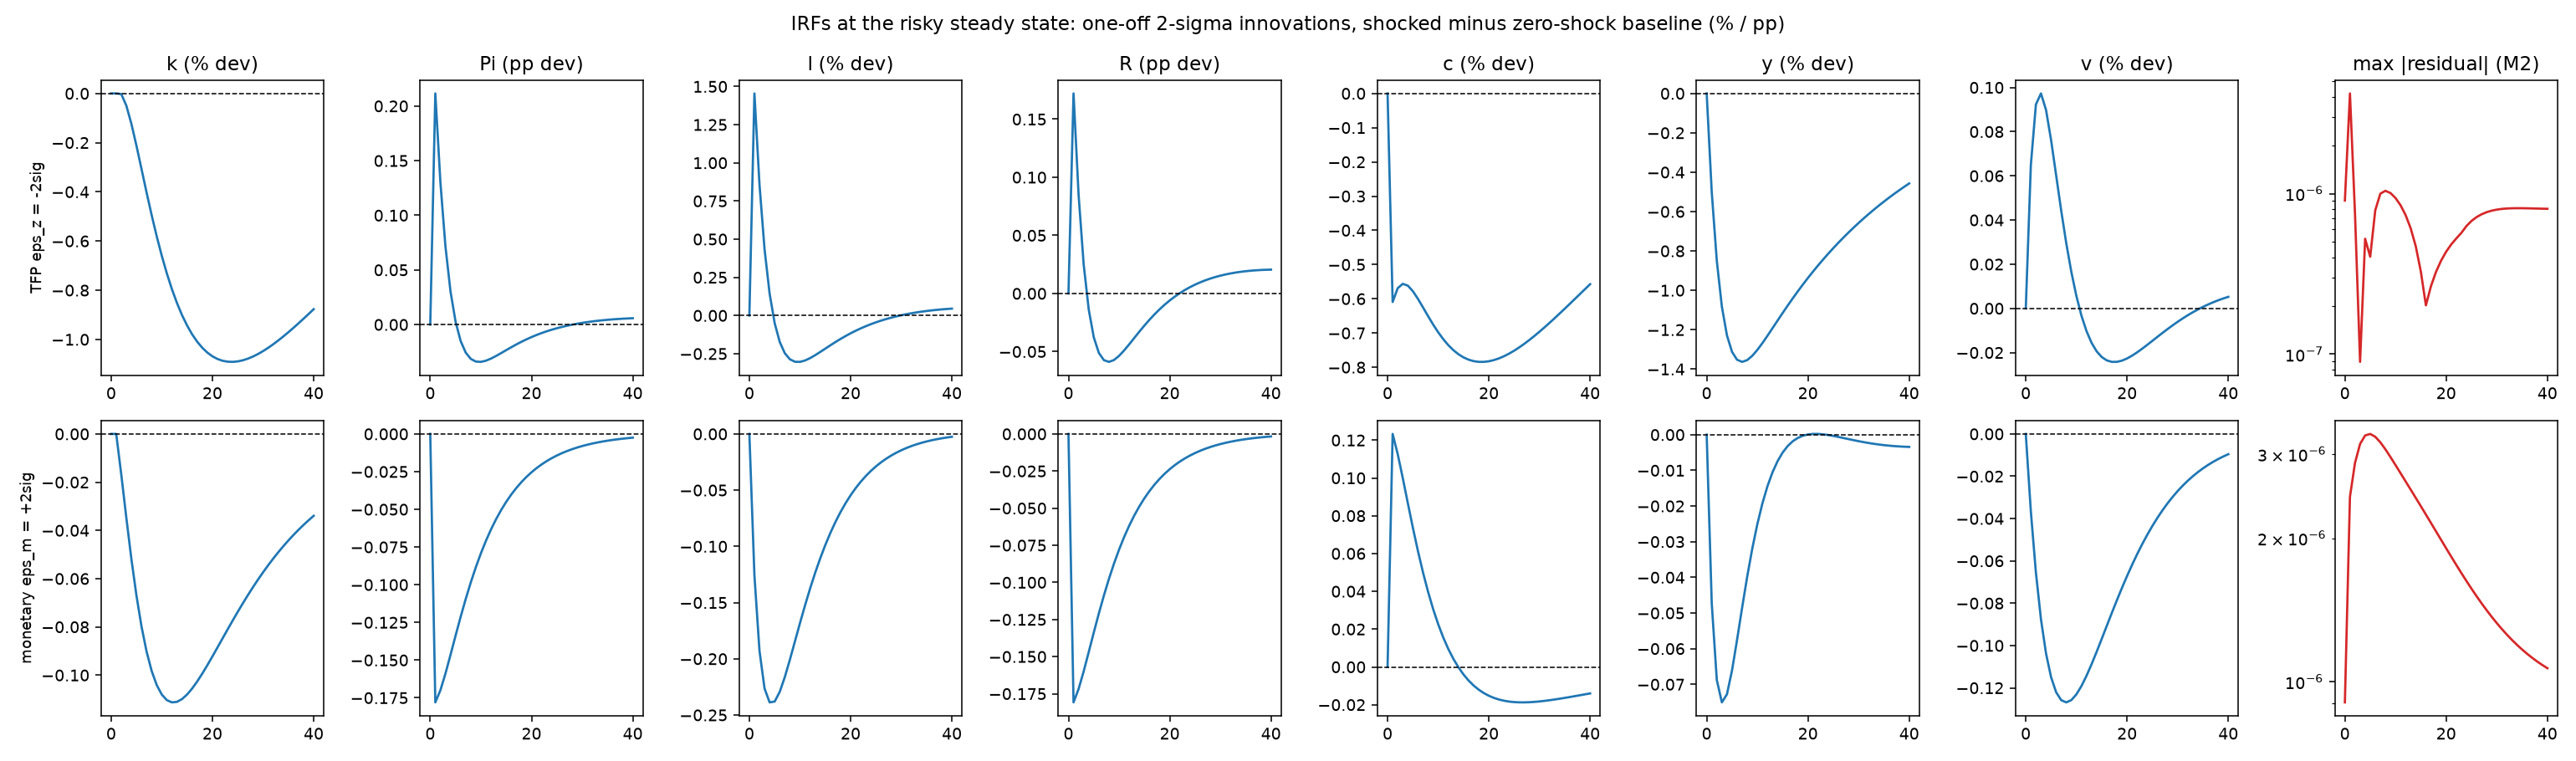
\includegraphics[width=\textwidth]{figures/calvo_irf.png}
\caption{Impulse responses of the stochastic policy at the risky steady state to one-off $2\sigma$ innovations (top: TFP, $\varepsilon_z = -2\sigma_z$; bottom: monetary, $\varepsilon_m = +2\sigma_m$), shocked minus zero-shock baseline, in percent or percentage points. The last column is the maximum absolute equilibrium residual over the four conditions, graded with the degree-5 monomial rule.}
\label{fig:irf}
\end{figure}

\paragraph{Stochastic policy: simulation.} Figure \ref{fig:sim} shows 36 simulated paths of 100 quarters from the risky steady state under the calibrated shocks, with the median per panel. Table \ref{tab:sim} summarizes the residuals. No path leaves the region where the model is well defined; inflation ranges from 0.994 to 1.013 against the singularity at 1.0236, price dispersion reaches 1.022, and capital moves between $0.92$ and $1.07$ times its steady-state value. The equilibrium residual has mean $3.5 \times 10^{-5}$ and median $7 \times 10^{-6}$ over the 3{,}600 simulated states, a 99th percentile of $4 \times 10^{-4}$, and a maximum of $1.3 \times 10^{-3}$, reached at the most extreme dispersion states, which lie at the edge of the resimulated clouds. 

\begin{figure}[htbp]
\centering
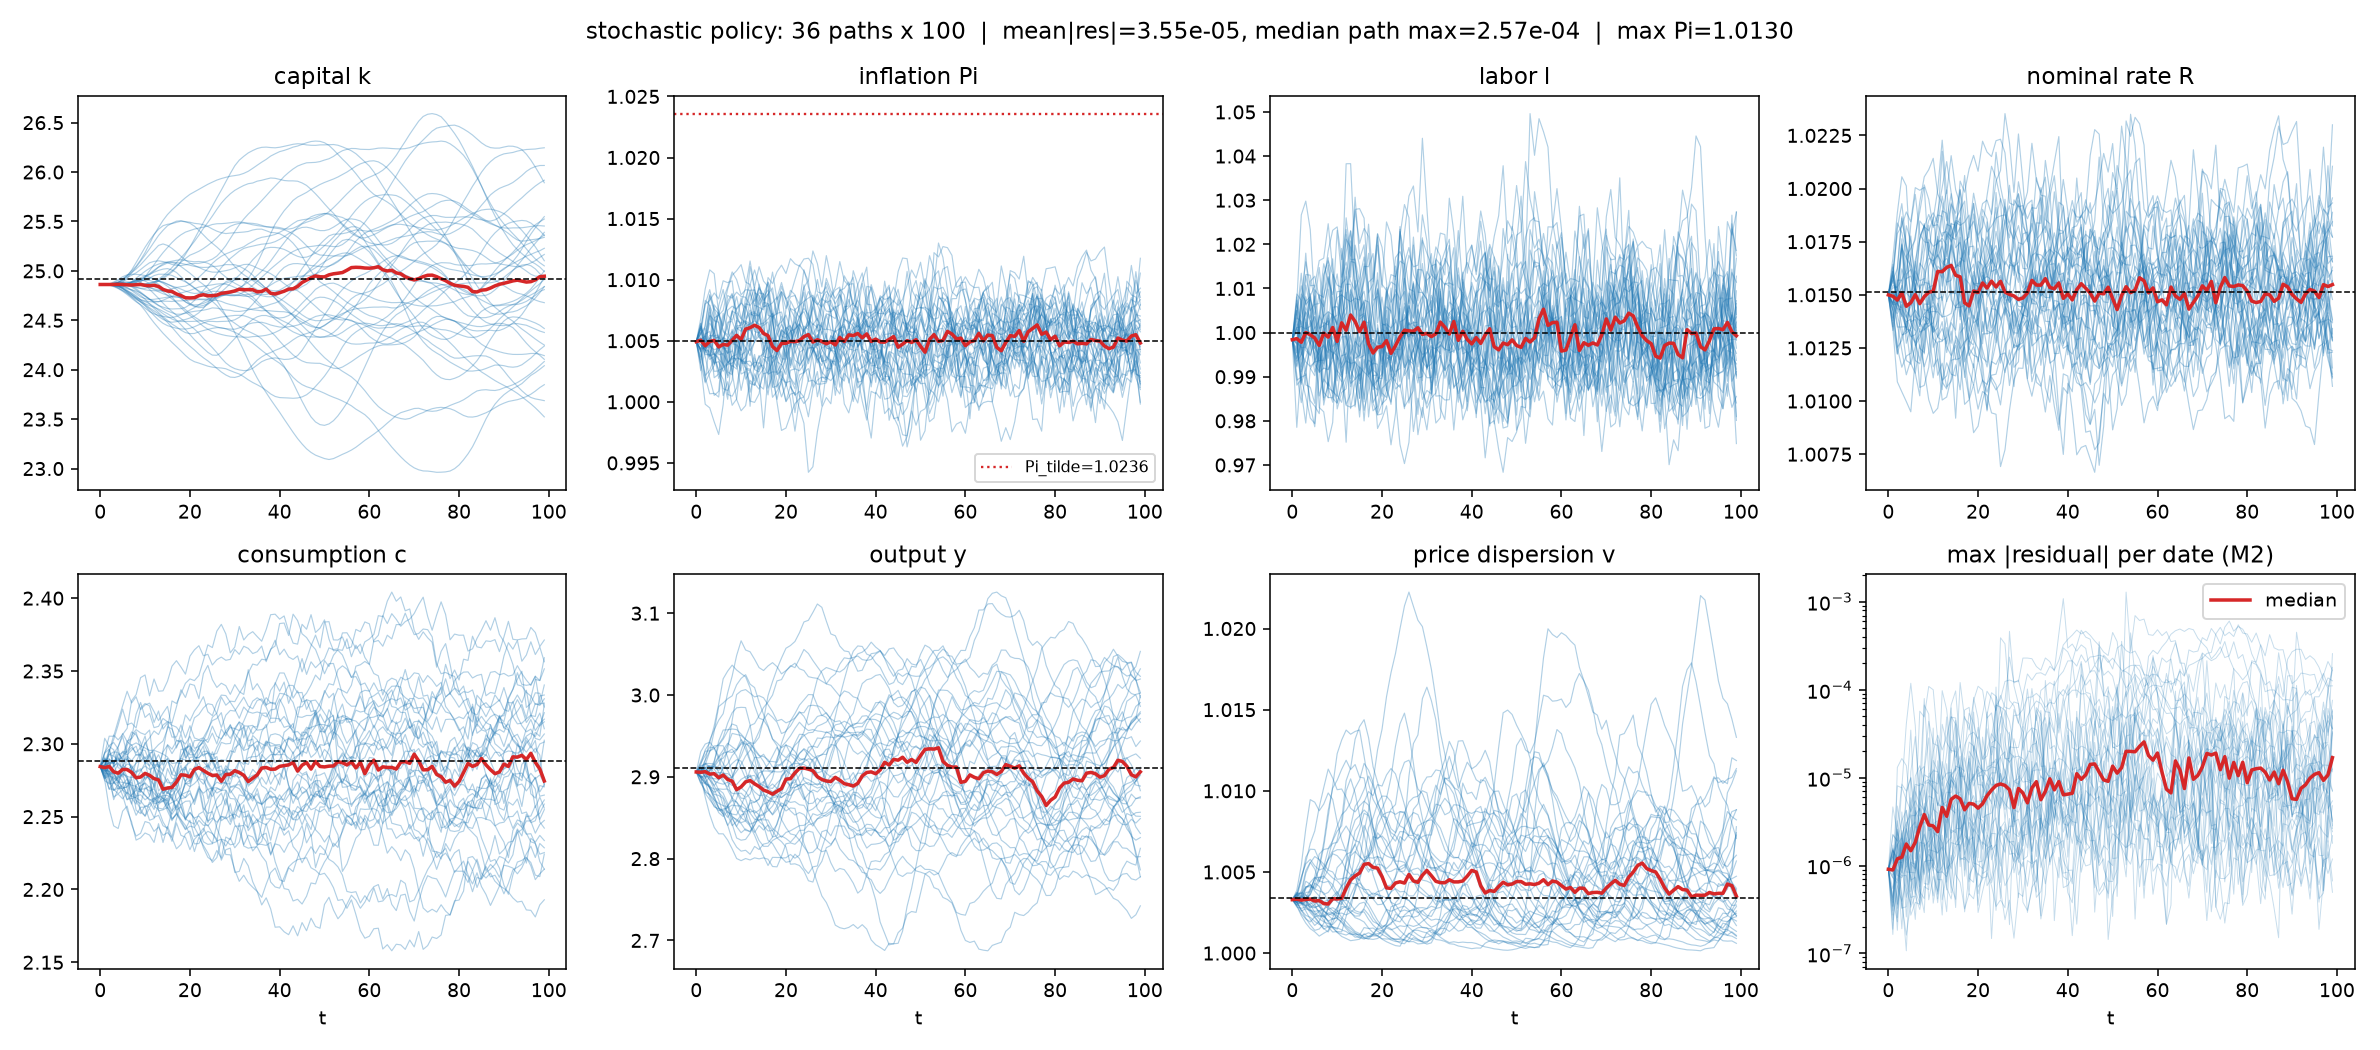
\includegraphics[width=\textwidth]{figures/calvo_sim.png}
\caption{Stochastic policy: 36 simulated paths of 100 quarters from the risky steady state under the calibrated shocks (blue), median per panel (red), deterministic steady state (dashed). The dotted line in the inflation panel is the singularity $\tilde\Pi$ of the Calvo block. The last panel is the per-date maximum absolute equilibrium residual.}
\label{fig:sim}
\end{figure}

\begin{table}[htbp]
\centering
\small
\begin{tabular}{lccccc}
\toprule
 & mean & median & p90 & p99 & max\\
\midrule
all four conditions, $\max_j |l_j(\sigma, f)(s)|$ & $3.5 \times 10^{-5}$ & $7.4 \times 10^{-6}$ & $9.6 \times 10^{-5}$ & $4.2 \times 10^{-4}$ & $1.3 \times 10^{-3}$\\
\midrule
bond Euler & $1.2 \times 10^{-5}$ & & & & $5.0 \times 10^{-4}$\\
capital Euler & $1.3 \times 10^{-5}$ & & & & $6.1 \times 10^{-4}$\\
marginal-cost recursion $g^1$ & $3.0 \times 10^{-5}$ & & & & $1.3 \times 10^{-3}$\\
revenue recursion $g^2$ & $2.3 \times 10^{-5}$ & & & & $8.8 \times 10^{-4}$\\
\bottomrule
\end{tabular}
\caption{Equilibrium residuals of the stochastic policy along the simulation of Figure \ref{fig:sim} (36 paths of 100 quarters, none dropped), graded with the nine-node degree-5 monomial rule. The per-row lines report the mean and the maximum of the absolute residual of each condition over the 3{,}600 simulated states.}
\label{tab:sim}
\end{table}


\bibliographystyle{ecta}
\bibliography{extended_abstract}

\end{document}
